%%%package list
\documentclass{article}
\usepackage[top=3cm, bottom=3cm, outer=3cm, inner=3cm]{geometry}
\usepackage{multicol}
\usepackage{graphicx}
\usepackage{url}

%\usepackage{cite}
\usepackage{hyperref}
\usepackage{array}
%\usepackage{multicol}
\newcolumntype{x}[1]{>{\centering\arraybackslash\hspace{0pt}}p{#1}}
\usepackage{natbib}
\usepackage{p	dfpages}
\usepackage{multirow}
\usepackage[normalem]{ulem}
\useunder{\uline}{\ul}{}
\usepackage{svg}
\usepackage{xcolor}
\usepackage{listings}
\lstdefinestyle{ascii-tree}{
    literate={├}{|}1 {─}{--}1 {└}{+}1 
  }
\lstset{basicstyle=\ttfamily,
  showstringspaces=false,
  commentstyle=\color{red},
  keywordstyle=\color{blue}
}

%\usepackage{booktabs}
\usepackage{caption}
\usepackage{subcaption}
\usepackage{float}
\usepackage{array}

\newcolumntype{M}[1]{>{\centering\arraybackslash}m{#1}}
\newcolumntype{N}{@{}m{0pt}@{}}

%%%%%%%%%%%%%%%%%%%%%%%%%%%%%%%%%%%%%%%%%%%%%%%%%%%%%%%%%%%%%%%%%%%%%%%%%%%%
%%%%%%%%%%%%%%%%%%%%%%%%%%%%%%%%%%%%%%%%%%%%%%%%%%%%%%%%%%%%%%%%%%%%%%%%%%%%
\newcommand{\itemEmail}{rttitoca@unsa.edu.pe}
\newcommand{\itemStudent}{Rutbel Carlos Ttito Campos}
\newcommand{\itemCourse}{Programación Web 2}
\newcommand{\itemCourseCode}{20231001}
\newcommand{\itemSemester}{III}
\newcommand{\itemUniversity}{Universidad Nacional de San Agustín de Arequipa}
\newcommand{\itemFaculty}{Facultad de Ingeniería de Producción y Servicios}
\newcommand{\itemDepartment}{Departamento Académico de Ingeniería de Sistemas e Informática}
\newcommand{\itemSchool}{Escuela Profesional de Ingeniería de Sistemas}
\newcommand{\itemAcademic}{2023 - A}
\newcommand{\itemInput}{Del 10 Abril 2023}
\newcommand{\itemOutput}{Al 17 Abril 2023}
\newcommand{\itemPracticeNumber}{04}
\newcommand{\itemTheme}{Python}
%%%%%%%%%%%%%%%%%%%%%%%%%%%%%%%%%%%%%%%%%%%%%%%%%%%%%%%%%%%%%%%%%%%%%%%%%%%%
%%%%%%%%%%%%%%%%%%%%%%%%%%%%%%%%%%%%%%%%%%%%%%%%%%%%%%%%%%%%%%%%%%%%%%%%%%%%

\usepackage[english,spanish]{babel}
\usepackage[utf8]{inputenc}
\AtBeginDocument{\selectlanguage{spanish}}
\renewcommand{\figurename}{Figura}
\renewcommand{\refname}{Referencias}
\renewcommand{\tablename}{Tabla} %esto no funciona cuando se usa babel
\AtBeginDocument{%
	\renewcommand\tablename{Tabla}
}

\usepackage{fancyhdr}
\pagestyle{fancy}
\fancyhf{}
\setlength{\headheight}{30pt}
\renewcommand{\headrulewidth}{1pt}
\renewcommand{\footrulewidth}{1pt}
\fancyhead[L]{\raisebox{-0.2\height}{
\includegraphics[width=3cm]{img/logo_episunsa.png}}}
\fancyhead[C]{\fontsize{7}{7}\selectfont	\itemUniversity \\ \itemFaculty \\ \itemDepartment \\ \itemSchool \\ \textbf{\itemCourse}}
\fancyhead[R]{\raisebox{-0.2\height}{
\includegraphics[width=1.2cm]{img/logo_abet.png}}}
\fancyfoot[L]{Est. \itemStudent}
\fancyfoot[C]{\itemCourse}
\fancyfoot[R]{Página \thepage}


% para el codigo fuente
\usepackage{listings}
\usepackage{color, colortbl}
\definecolor{dkgreen}{rgb}{0,0.6,0}
\definecolor{gray}{rgb}{0.5,0.5,0.5}
\definecolor{mauve}{rgb}{0.58,0,0.82}
\definecolor{codebackground}{rgb}{0.95, 0.95, 0.92}
\definecolor{tablebackground}{rgb}{0.8, 0, 0}

\lstset{frame=tb,
    language=bash,
    aboveskip=3mm,
    belowskip=3mm,
    showstringspaces=false,
    columns=flexible,
    basicstyle={\small\ttfamily},
    numbers=none,
    numberstyle=\tiny\color{gray},
    keywordstyle=\color{blue},
    commentstyle=\color{dkgreen},
    stringstyle=\color{mauve},
    breaklines=true,
    breakatwhitespace=true,
    tabsize=3,
    backgroundcolor= \color{codebackground},
}



\usepackage{graphicx} % Required for inserting images

\begin{document}

\vspace*{10px}

\begin{center}
	\fontsize{17}{17} \textbf{ Informe de Laboratorio \itemPracticeNumber}
\end{center}
\centerline{\textbf{\Large Tema: \itemTheme}}
%\vspace*{0.5cm}	

\begin{flushright}
	\begin{tabular}{|M{2.5cm}|N|}
		\hline
		\rowcolor{tablebackground}
		\color{white} \textbf{Nota} \\
		\hline
		\\[30pt]
		\hline
	\end{tabular}
\end{flushright}

\begin{table}[H]
	\begin{tabular}{|x{4.7cm}|x{4.8cm}|x{4.8cm}|}
		\hline
		\rowcolor{tablebackground}
		\color{white} \textbf{Estudiante} & \color{white}\textbf{Escuela} & \color{white}\textbf{Asignatura}                                        \\
		\hline
		{\itemStudent \par \itemEmail}    & \itemSchool                   & {\itemCourse \par Semestre: \itemSemester \par Código: \itemCourseCode} \\
		\hline
	\end{tabular}
\end{table}

\begin{table}[H]
	\begin{tabular}{|x{4.7cm}|x{4.8cm}|x{4.8cm}|}
		\hline
		\rowcolor{tablebackground}
		\color{white}\textbf{Laboratorio} & \color{white}\textbf{Tema} & \color{white}\textbf{Duración} \\
		\hline
		\itemPracticeNumber               & \itemTheme                 & 04 horas                       \\
		\hline
	\end{tabular}
\end{table}

\begin{table}[H]
	\begin{tabular}{|x{4.7cm}|x{4.8cm}|x{4.8cm}|}
		\hline
		\rowcolor{tablebackground}
		\color{white}\textbf{Semestre académico} & \color{white}\textbf{Fecha de inicio} & \color{white}\textbf{Fecha de entrega} \\
		\hline
		\itemAcademic                            & \itemInput                            & \itemOutput                            \\
		\hline
	\end{tabular}
\end{table}

\section{Equipos, materiales y temas utilizados}
\begin{itemize}
	\item Sistema Operativo Ubuntu 22.04.2 LTS
	\item Git 2.39.2.
	\item Cuenta en GitHub con el correo institucional.
	\item Python
	\item Arreglos en python
\end{itemize}

\section{Tarea}
\begin{itemize}
	\item URL GitHub de Tarea del Ajedrez \url{https://github.com/rescobedoq/pw2/tree/main/labs/lab04/Tarea-del-Ajedrez}
	\item En esta tarea usted pondrá en práctica sus conocimientos de programación en Python para dibujar un tablero de Ajedrez.
	\item La parte gráfica ya está programada, usted sólo tendrá que concentrarse en las estructuras de datos subyacentes.
	\item Con el código proporcionado usted dispondrá de varios objetos de tipo Picture para poder realizar su tarea:
	      \begin{center}
		      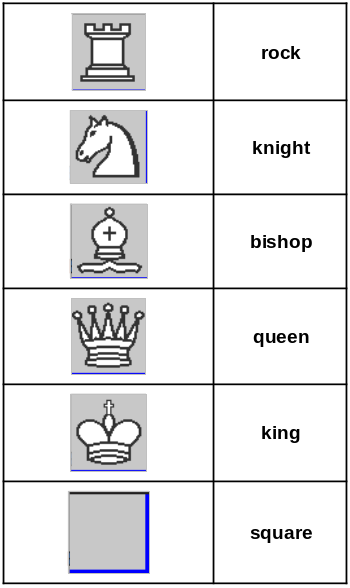
\includegraphics[width=154.679pt,height=259.8607pt]{img/piezas.png}
	      \end{center}
	\item Ejercicios:
	      \begin{itemize}
		      \item Para resolver los siguientes ejercicios sólo está permitido usar ciclos, condicionales, definición de listas por comprensión, sublistas, map, join, (+), lambda, zip, append, pop, range.
		      \item Implemente los métodos de la clase Picture. Se recomienda que implemente la clase picture por etapas, probando realizar los dibujos que se muestran en la siguiente preguntas.
		      \item Usando únicamente los métodos de los objetos de la clase Picture dibuje las siguientes figuras (invoque a draw):
		            \begin{itemize}
			            \item ejercicio a
			                  \begin{center}
				                  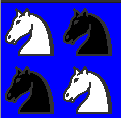
\includegraphics[width=154.719pt,height=150.883pt]{img/ejercicio_02_a.png}
			                  \end{center}

			            \item ejercicio b
			                  \begin{center}
				                  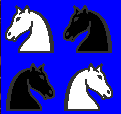
\includegraphics[width=154.719pt,height=145.7683pt]{img/ejercicio_02_b.png}
			                  \end{center}

			            \item ejercicio c
			                  \begin{center}
				                  
\includegraphics[width=154.6881pt,height=37.17827pt]{img/ejercicio_02_c.png}
			                  \end{center}

			            \item ejercicio d
			                  \begin{center}
				                  
\includegraphics[width=154.6824pt,height=19.04297pt]{img/ejercicio_02_d.png}
			                  \end{center}

			            \item ejercicio e
			                  \begin{center}
				                  
\includegraphics[width=154.6776pt,height=18.96048pt]{img/ejercicio_02_e.png}
			                  \end{center}

			            \item ejercicio f
			                  \begin{center}
				                  
\includegraphics[width=154.6881pt,height=77.01212pt]{img/ejercicio_02_f.png}
			                  \end{center}

			            \item ejercicio g
			                  \begin{center}
				                  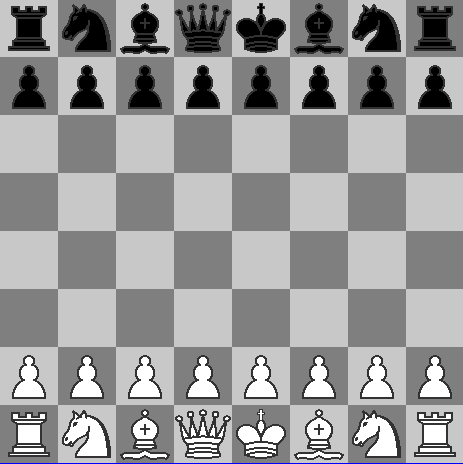
\includegraphics[width=154.6824pt,height=155.0165pt]{img/ejercicio_02_g.png}
			                  \end{center}
		            \end{itemize}
	      \end{itemize}
\end{itemize}
\section{Solucion de Ejercicios}
\subsection{Creando entorno virtual}
\begin{center}
	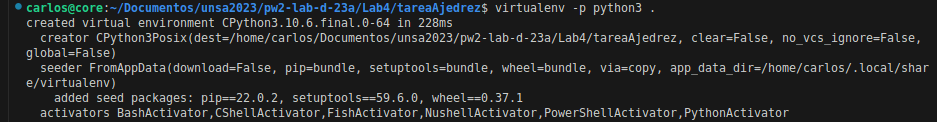
\includegraphics[scale=0.45]{img/entornoVirtual.png}
\end{center}

\subsection{Instalando Pygame}
\begin{center}
	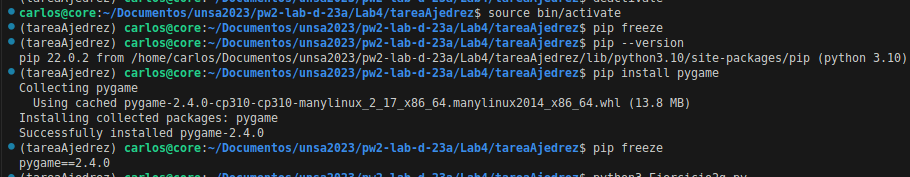
\includegraphics[scale=0.45]{img/Pygame.png}
\end{center}

\subsection{Funciones de la clase Picture}
\lstinputlisting[language=Python, caption={picture.py},numbers=left,]{src/picture.py}

\subsection{Ejercicios}
\lstinputlisting[language=Python, caption={Ejercicio2a.py},numbers=left,]{src/Ejercicio2a.py}
\lstinputlisting[language=Python, caption={Ejercicio2b.py},numbers=left,]{src/Ejercicio2b.py}
\lstinputlisting[language=Python, caption={Ejercicio2c.py},numbers=left,]{src/Ejercicio2c.py}
\lstinputlisting[language=Python, caption={Ejercicio2d.py},numbers=left,]{src/Ejercicio2d.py}
\lstinputlisting[language=Python, caption={Ejercicio2e.py},numbers=left,]{src/Ejercicio2e.py}
\lstinputlisting[language=Python, caption={Ejercicio2f.py},numbers=left,]{src/Ejercicio2f.py}
\lstinputlisting[language=Python, caption={Ejercicio2g.py},numbers=left,]{src/Ejercicio2g.py}

\subsection{Capturas de Ejecucion}
\begin{figure}[H]
    \centering
    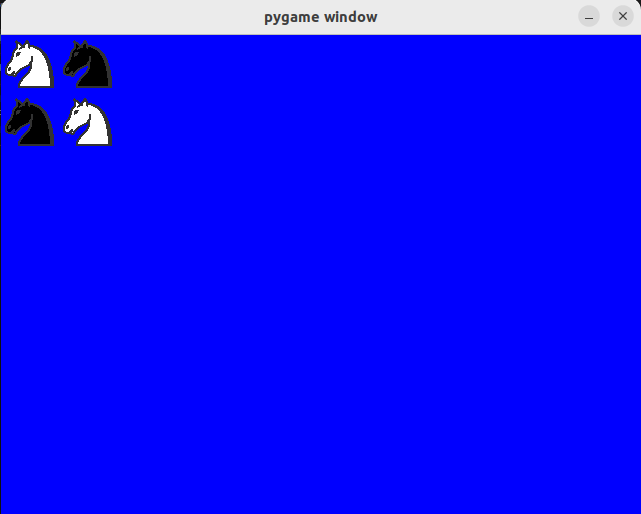
\includegraphics[scale=0.3]{img/capturaEjercicio2a.png}
    \caption{ejecucion ejercicio a}
\end{figure}
\begin{figure}[H]
    \centering
    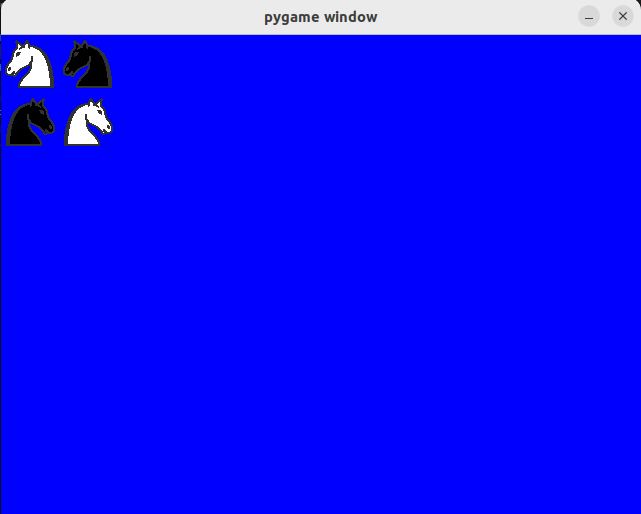
\includegraphics[scale=0.3]{img/capturaEjercicio2b.png}
    \caption{ejecucion ejercicio b}
\end{figure}
\begin{figure}[H]
    \centering
    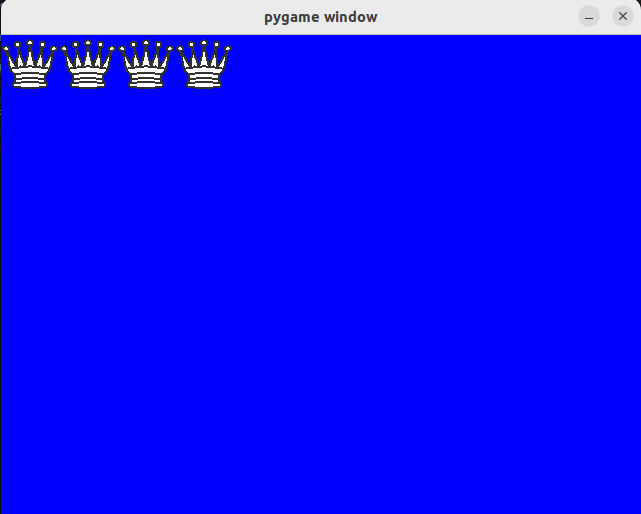
\includegraphics[scale=0.3]{img/capturaEjercicio2c.png}
    \caption{ejecucion ejercicio c}
\end{figure}
\begin{figure}[H]
    \centering
    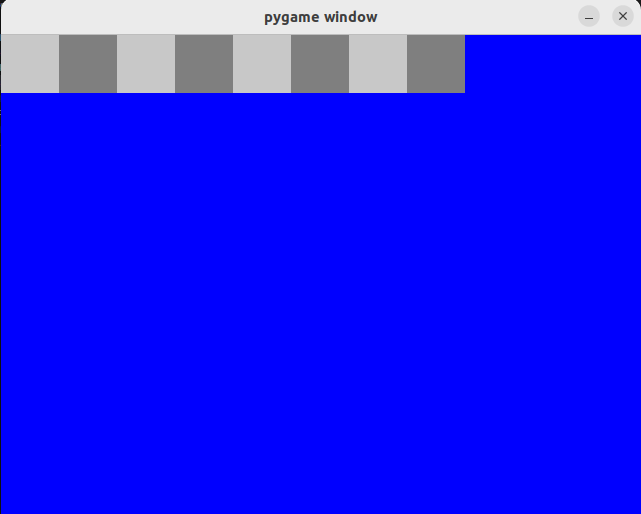
\includegraphics[scale=0.3]{img/capturaEjercicio2d.png}
    \caption{ejecucion ejercicio d}
\end{figure}
\begin{figure}[H]
    \centering
    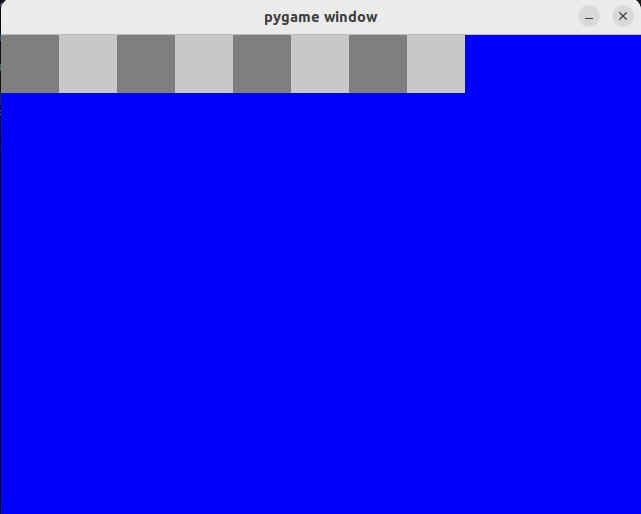
\includegraphics[scale=0.3]{img/capturaEjercicio2e.png}
    \caption{ejecucion ejercicio e}
\end{figure}
\begin{figure}[H]
    \centering
    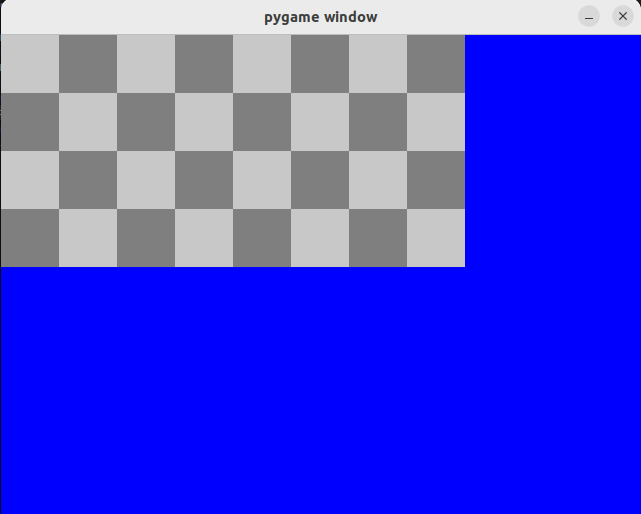
\includegraphics[scale=0.3]{img/capturaEjercicio2f.png}
    \caption{ejecucion ejercicio f}
\end{figure}
%%%%%%%%%%%%%%%%%%%%%%%%%%%%%%%%%%%%%%%%%%%%%%%%%%%%%%%%%
\begin{figure}[H]
    \centering
    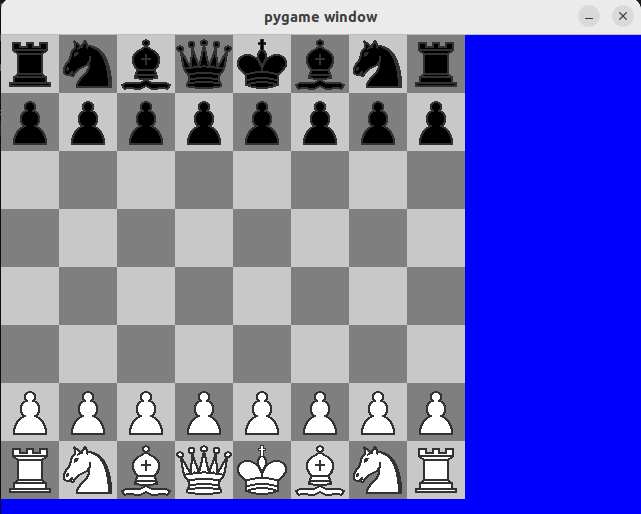
\includegraphics[scale=0.3]{img/capturaEjercicio2g.png}
    \caption{ejecucion ejercicio g}
\end{figure}
%%%%%%%%%




\section{URL de Repositorio Github}
\begin{itemize}
	\item URL del Repositorio GitHub para clonar o recuperar:
	\item \url{https://github.com/RutbelCarlosTC/pw2-lab-d-23a.git}
	\item URL para el laboratorio 04 en el Repositorio GitHub.
	\item \url{https://github.com/RutbelCarlosTC/pw2-lab-d-23a/tree/main/Lab4}
\end{itemize}

\section{Actividades con el repositorio GitHub}

\subsection{Commits}
\begin{itemize}
	\item Primer commit agregando carpeta con plantillas de ejercicios de Tarea-del-Ajedrez
	      \begin{center}
		      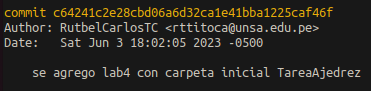
\includegraphics[]{img/commits/commit-ajedrez.png}
	      \end{center}
	\item Agregando archivo .gitignore
	      \begin{center}
		      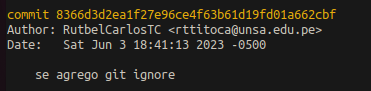
\includegraphics[]{img/commits/commit-gitignore.png}
	      \end{center}
    %%%%%%%%%%%
    \item Completando funciones
    \begin{figure}[H]
        \centering
        \begin{subfigure}[b]{0.4\textwidth}
          \centering
          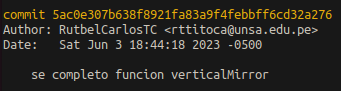
\includegraphics[scale=0.5]{img/commits/verticalMirror.png}
          \caption{verticalMirror}
        \end{subfigure}
        \hfill
        \begin{subfigure}[b]{0.4\textwidth}
          \centering
          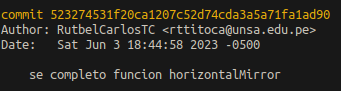
\includegraphics[scale=0.5]{img/commits/horizontalMirror.png}
          \caption{horizontalMirror}
        \end{subfigure}
        
        \vspace{0.5cm} % Espacio vertical entre los grupos de imágenes
        
        \begin{subfigure}[b]{0.4\textwidth}
          \centering
          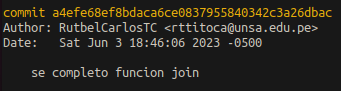
\includegraphics[scale=0.5]{img/commits/join.png}
          \caption{join}
        \end{subfigure}
        \hfill
        \begin{subfigure}[b]{0.4\textwidth}
          \centering
          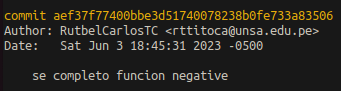
\includegraphics[scale=0.5]{img/commits/negative.png}
          \caption{Negative}
        \end{subfigure}
        
        \vspace{0.5cm} % Espacio vertical entre los grupos de imágenes
        
        \begin{subfigure}[b]{0.4\textwidth}
          \centering
          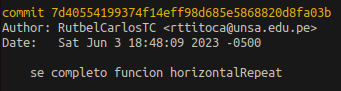
\includegraphics[scale=0.5]{img/commits/horizontalRepeat.png}
          \caption{horizontalRepeat}
        \end{subfigure}
        \hfill
        \begin{subfigure}[b]{0.4\textwidth}
          \centering
          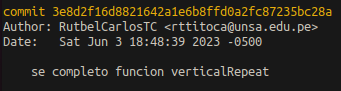
\includegraphics[scale=0.5]{img/commits/verticalRepeat.png}
          \caption{verticalRepeat}
        \end{subfigure}
  
        \vspace{0.5cm}
        
        \begin{subfigure}[b]{0.4\textwidth}
          \centering
          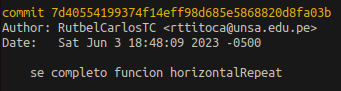
\includegraphics[scale=0.5]{img/commits/horizontalRepeat.png}
          \caption{horizontalRepeat}
        \end{subfigure}
        \hfill
        \begin{subfigure}[b]{0.4\textwidth}
          \centering
          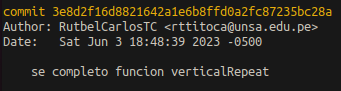
\includegraphics[scale=0.5]{img/commits/verticalRepeat.png}
          \caption{verticalRepeat}
        \end{subfigure}
  
      \end{figure}
    %%%%%

    \item Completando ejercicios:
    \begin{figure}[H]
      \centering
      \begin{subfigure}[b]{0.4\textwidth}
        \centering
        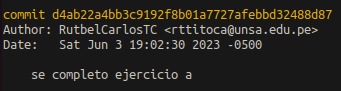
\includegraphics[width=\textwidth]{img/commits/commitEjer-a.png}
        \caption{Commit Ejercicio a}
      \end{subfigure}
      \hfill
      \begin{subfigure}[b]{0.4\textwidth}
        \centering
        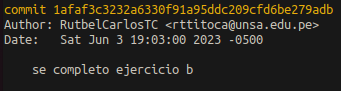
\includegraphics[width=\textwidth]{img/commits/commitEjer-b.png}
        \caption{Commit Ejercicio b}
      \end{subfigure}
      
      \vspace{0.5cm} % Espacio vertical entre los grupos de imágenes
      
      \begin{subfigure}[b]{0.4\textwidth}
        \centering
        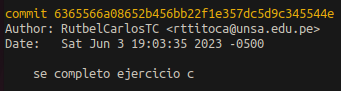
\includegraphics[width=\textwidth]{img/commits/commitEjer-c.png}
        \caption{Commit Ejercicio c}
      \end{subfigure}
      \hfill
      \begin{subfigure}[b]{0.4\textwidth}
        \centering
        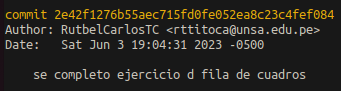
\includegraphics[width=\textwidth]{img/commits/commitEjer-d.png}
        \caption{Commit Ejercicio d}
      \end{subfigure}
      
      \vspace{0.5cm} % Espacio vertical entre los grupos de imágenes
      
      \begin{subfigure}[b]{0.4\textwidth}
        \centering
        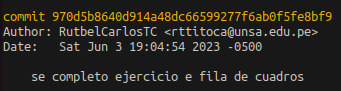
\includegraphics[width=\textwidth]{img/commits/commitEjer-e.png}
        \caption{Commit Ejercicio e}
      \end{subfigure}
      \hfill
      \begin{subfigure}[b]{0.4\textwidth}
        \centering
        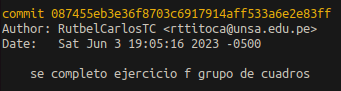
\includegraphics[width=\textwidth]{img/commits/commitEjer-f.png}
        \caption{Commit Ejercicio f}
      \end{subfigure}

      \vspace{0.5cm}
      
      \begin{subfigure}[b]{0.4\textwidth}
        \centering
        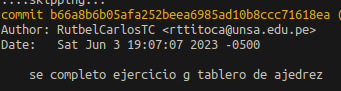
\includegraphics[width=\textwidth]{img/commits/commitEjer-g.png}
        \caption{Commit Ejercicio g}
      \end{subfigure}

    \end{figure}
        
\end{itemize}

%%%%%%%%%%%%%%%%%%%%%%%%%%%%%
\section{Pregunta: ¿Para qué sirve el directorio pycache?}
Se utiliza para almacenar los archivos de código compilado en formato de bytecode de Python (*.pyc) para mejorar el rendimiento en futuras ejecuciones.


\section{\textcolor{red}{Rúbricas}}
\subsection{\textcolor{red}{Entregable Informe}}
\begin{table}[H]
	\caption{Tipo de Informe}
	\setlength{\tabcolsep}{0.5em} % for the horizontal padding
	{\renewcommand{\arraystretch}{1.5}% for the vertical padding

		\begin{tabular}{|p{3cm}|p{12cm}|}
			\hline
			\multicolumn{2}{|c|}{\textbf{\textcolor{red}{Informe}}}                                                                                                      \\
			\hline
			\textbf{\textcolor{red}{Latex}} & \textcolor{blue}{El informe está en formato PDF desde Latex,  con un formato limpio (buena presentación) y facil de leer.} \\
			\hline
		\end{tabular}
	}
\end{table}

\clearpage

\subsection{\textcolor{red}{Rúbrica para el contenido del Informe y demostración}}

\begin{itemize}
	\item El alumno debe marcar o dejar en blanco en celdas de la columna \textbf{Checklist} si cumplio con el ítem correspondiente.
	\item Si un alumno supera la fecha de entrega,  su calificación será sobre la nota mínima aprobada, siempre y cuando cumpla con todos lo items.
	\item El alumno debe autocalificarse en la columna \textbf{Estudiante} de acuerdo a la siguiente tabla:

	      \begin{table}[ht]
		      \caption{Niveles de desempeño}
		      \begin{center}
			      \begin{tabular}{ccccc}
				      \hline
				                      & \multicolumn{4}{c}{Nivel}                                                              \\
				      \cline{1-5}
				      \textbf{Puntos} & Insatisfactorio 25\%      & En Proceso 50\% & Satisfactorio 75\% & Sobresaliente 100\% \\
				      \textbf{2.0}    & 0.5                       & 1.0             & 1.5                & 2.0                 \\
				      \textbf{4.0}    & 1.0                       & 2.0             & 3.0                & 4.0                 \\
				      \hline
			      \end{tabular}
		      \end{center}
	      \end{table}

\end{itemize}

\begin{table}[H]
	\caption{Rúbrica para contenido del Informe y demostración}
	\setlength{\tabcolsep}{0.5em} % for the horizontal padding
	{\renewcommand{\arraystretch}{1.5}% for the vertical padding
		%\begin{center}
		\begin{tabular}{|p{2.7cm}|p{7cm}|x{1.3cm}|p{1.2cm}|p{1.5cm}|p{1.1cm}|}
			\hline
			\multicolumn{2}{|c|}{Contenido y demostración} & Puntos                                                                                                                                                                                                          & Checklist & Estudiante & Profesor   \\
			\hline
			\textbf{1. GitHub}                             & Hay enlace URL activo del directorio para el  laboratorio hacia su repositorio GitHub con código fuente terminado y fácil de revisar.                                                                           & 2         & X          & 2        & \\
			\hline
			\textbf{2. Commits}                            & Hay capturas de pantalla de los commits más importantes con sus explicaciones detalladas. (El profesor puede preguntar para refrendar calificación).                                                            & 4         & X          & 3         & \\
			\hline
			\textbf{3. Código fuente}                      & Hay porciones de código fuente importantes con numeración y explicaciones detalladas de sus funciones.                                                                                                          & 2         & X          & 2        & \\
			\hline
			\textbf{4. Ejecución}                          & Se incluyen ejecuciones/pruebas del código fuente  explicadas gradualmente.                                                                                                                                     & 2         & X          & 2        & \\
			\hline
			\textbf{5. Pregunta}                           & Se responde con completitud a la pregunta formulada en la tarea.  (El profesor puede preguntar para refrendar calificación).                                                                                    & 2         & X          & 2        & \\
			\hline
			\textbf{6. Fechas}                             & Las fechas de modificación del código fuente estan dentro de los plazos de fecha de entrega establecidos.                                                                                                       & 2         & X          & 2        & \\
			\hline
			\textbf{7. Ortografía}                         & El documento no muestra errores ortográficos.                                                                                                                                                                   & 2         & X          & 1        & \\
			\hline
			\textbf{8. Madurez}                            & El Informe muestra de manera general una evolución de la madurez del código fuente,  explicaciones puntuales pero precisas y un acabado impecable.   (El profesor puede preguntar para refrendar calificación). & 4         & X           & 3        & \\
			\hline
			\multicolumn{2}{|c|}{\textbf{Total}}           & 20                                                                                                                                                                                                              &           & 17         &          \\
			\hline
		\end{tabular}
		%\end{center}
		%\label{tab:multicol}
	}
\end{table}

\clearpage

\section{Referencias}
\begin{itemize}
	\item \url{https://www.w3schools.com/java/default.asp}
	\item \url{https://www.geeksforgeeks.org/insertion-sort/}
\end{itemize}


\end{document}
